\documentclass{extbook}[14pt]
\usepackage{multicol, enumerate, enumitem, hyperref, color, soul, setspace, parskip, fancyhdr, amssymb, amsthm, amsmath, bbm, latexsym, units, mathtools}
\everymath{\displaystyle}
\usepackage[headsep=0.5cm,headheight=0cm, left=1 in,right= 1 in,top= 1 in,bottom= 1 in]{geometry}
\usepackage{dashrule}  % Package to use the command below to create lines between items
\newcommand{\litem}[1]{\item #1

\rule{\textwidth}{0.4pt}}
\pagestyle{fancy}
\lhead{}
\chead{Answer Key for FinalExam Version A}
\rhead{}
\lfoot{4952-8460}
\cfoot{}
\rfoot{Makeup Early Exam}
\begin{document}
\textbf{This key should allow you to understand why you choose the option you did (beyond just getting a question right or wrong). \href{https://xronos.clas.ufl.edu/mac1105spring2020/courseDescriptionAndMisc/Exams/LearningFromResults}{More instructions on how to use this key can be found here}.}

\textbf{If you have a suggestion to make the keys better, \href{https://forms.gle/CZkbZmPbC9XALEE88}{please fill out the short survey here}.}

\textit{Note: This key is auto-generated and may contain issues and/or errors. The keys are reviewed after each exam to ensure grading is done accurately. If there are issues (like duplicate options), they are noted in the offline gradebook. The keys are a work-in-progress to give students as many resources to improve as possible.}

\rule{\textwidth}{0.4pt}

\begin{enumerate}\litem{
Construct the lowest-degree polynomial given the zeros below. Then, choose the intervals that contain the coefficients of the polynomial in the form $ax^3+bx^2+cx+d$.
\[ 4, \frac{2}{3}, \text{ and } \frac{1}{4} \]

The solution is \( 12x^{3} -59 x^{2} +46 x -8 \), which is option D.\begin{enumerate}[label=\Alph*.]
\item \( a \in [11, 20], b \in [-64, -52], c \in [37, 51], \text{ and } d \in [6, 12] \)

$12x^{3} -59 x^{2} +46 x + 8$, which corresponds to multiplying everything correctly except the constant term.
\item \( a \in [11, 20], b \in [35, 42], c \in [-48, -34], \text{ and } d \in [6, 12] \)

$12x^{3} +37 x^{2} -42 x + 8$, which corresponds to multiplying out $(x + 4)(3x -2)(4x -1)$.
\item \( a \in [11, 20], b \in [57, 67], c \in [37, 51], \text{ and } d \in [6, 12] \)

$12x^{3} +59 x^{2} +46 x + 8$, which corresponds to multiplying out $(x + 4)(3x + 2)(4x + 1)$.
\item \( a \in [11, 20], b \in [-64, -52], c \in [37, 51], \text{ and } d \in [-11, -6] \)

* $12x^{3} -59 x^{2} +46 x -8$, which is the correct option.
\item \( a \in [11, 20], b \in [51, 57], c \in [16, 20], \text{ and } d \in [-11, -6] \)

$12x^{3} +53 x^{2} +18 x -8$, which corresponds to multiplying out $(x + 4)(3x + 2)(4x -1)$.
\end{enumerate}

\textbf{General Comment:} To construct the lowest-degree polynomial, you want to multiply out $(x -4)(3x -2)(4x -1)$
}
\litem{
Choose the graph of the equation below.
\[ f(x) = \sqrt{x + 10} + 3 \]

The solution is the graph below, which is option C.
\begin{center}
    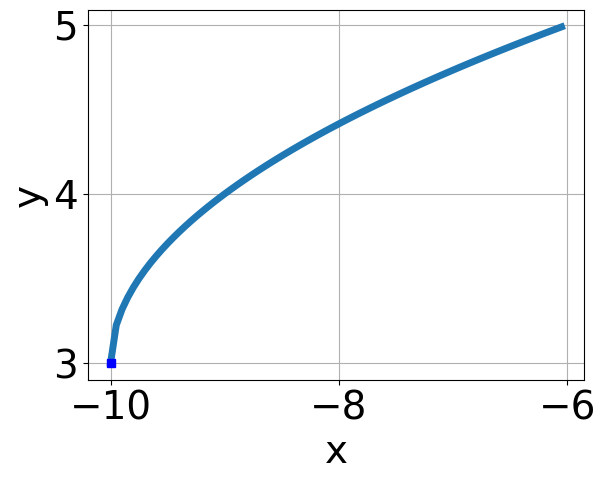
\includegraphics[width=0.3\textwidth]{../Figures/radicalEquationToGraphCA.png}
\end{center}\begin{enumerate}[label=\Alph*.]
\begin{multicols}{2}
\item 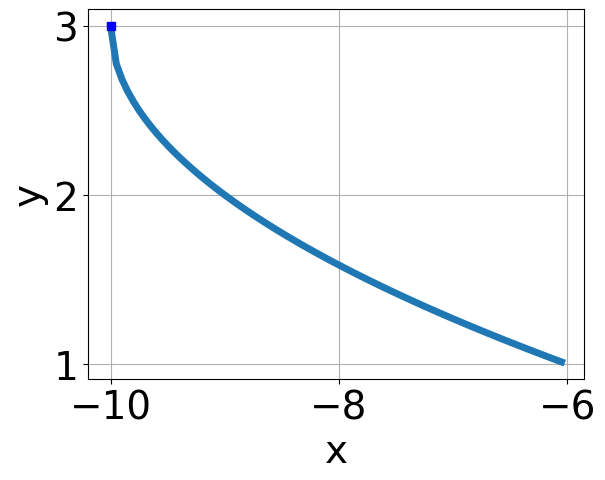
\includegraphics[width = 0.3\textwidth]{../Figures/radicalEquationToGraphAA.png}
\item 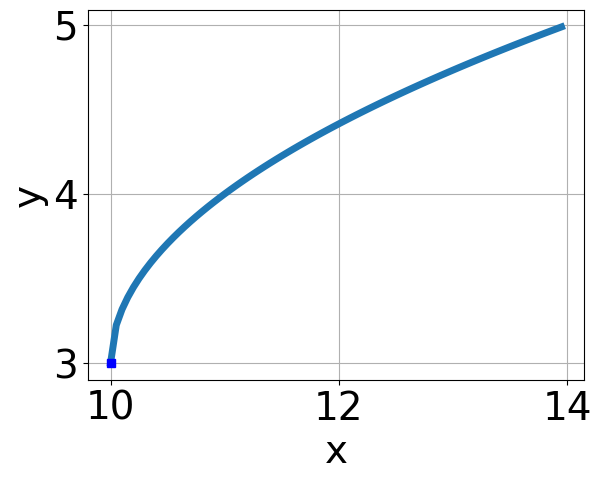
\includegraphics[width = 0.3\textwidth]{../Figures/radicalEquationToGraphBA.png}
\item 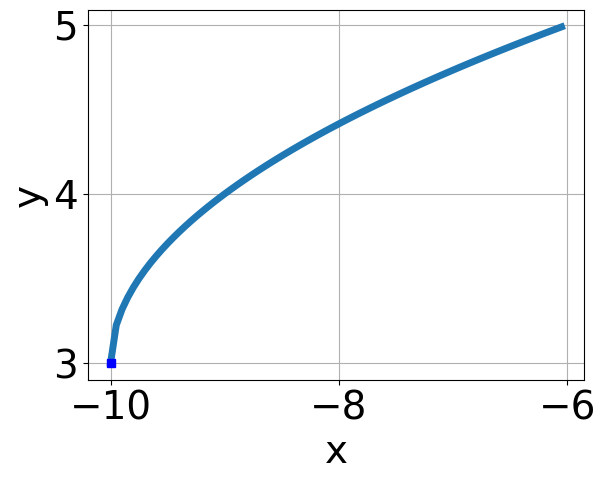
\includegraphics[width = 0.3\textwidth]{../Figures/radicalEquationToGraphCA.png}
\item 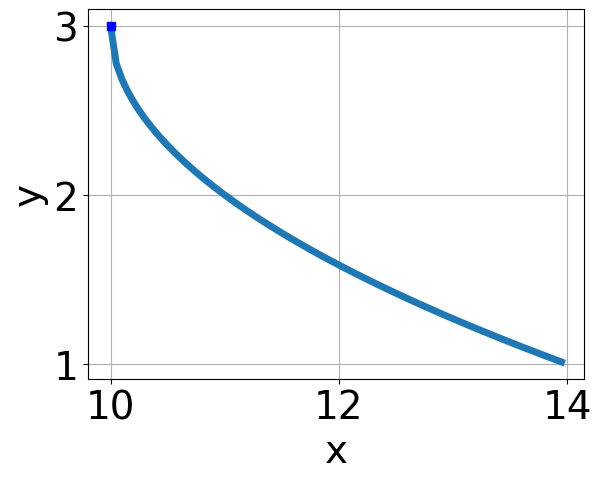
\includegraphics[width = 0.3\textwidth]{../Figures/radicalEquationToGraphDA.png}
\end{multicols}\item None of the above.\end{enumerate}
\textbf{General Comment:} Remember that the general form of a radical equation is $ f(x) = a \sqrt[b]{x - h} + k $, where $a$ is the leading coefficient (and in this case, we assume is either 1 or -1), $b$ is the root degree (in this case, either 2 or 3), and $(h, k)$ is the vertex.
}
\litem{
Which of the following equations \textit{could} be of the graph presented below?

\begin{center}
    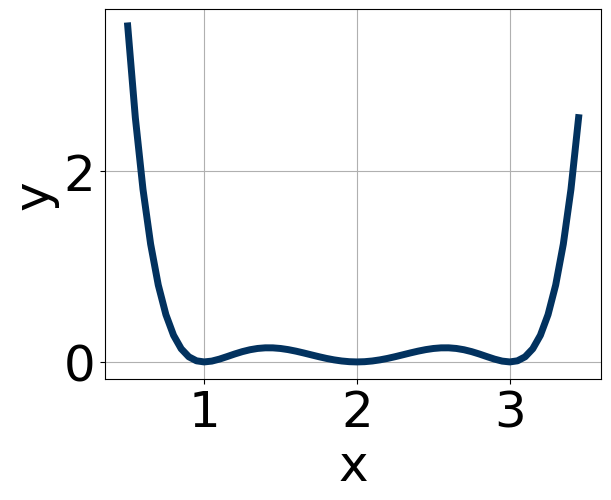
\includegraphics[width=0.5\textwidth]{../Figures/polyGraphToFunctionA.png}
\end{center}




The solution is \( 17(x - 2)^{8} (x - 1)^{6} (x - 3)^{6} \), which is option A.\begin{enumerate}[label=\Alph*.]
\item \( 17(x - 2)^{8} (x - 1)^{6} (x - 3)^{6} \)

* This is the correct option.
\item \( 13(x - 2)^{8} (x - 1)^{11} (x - 3)^{7} \)

The factors $(x - 1)$ and $(x - 3)$ should both have even powers.
\item \( 15(x - 2)^{4} (x - 1)^{4} (x - 3)^{9} \)

The factor $(x - 3)$ should have an even power.
\item \( -15(x - 2)^{10} (x - 1)^{10} (x - 3)^{4} \)

This corresponds to the leading coefficient being the opposite value than it should be.
\item \( -16(x - 2)^{4} (x - 1)^{6} (x - 3)^{11} \)

The factor $(x - 3)$ should have an even power and the leading coefficient should be the opposite sign.
\end{enumerate}

\textbf{General Comment:} General Comments: Draw the x-axis to determine which zeros are touching (and so have even multiplicity) or cross (and have odd multiplicity).
}
\litem{
Solve the radical equation below. Then, choose the interval(s) that the solution(s) belongs to.
\[ \sqrt{-6 x - 5} - \sqrt{7 x - 9} = 0 \]

The solution is \( \text{All solutions lead to invalid or complex values in the equation.} \), which is option A.\begin{enumerate}[label=\Alph*.]
\item \( \text{All solutions lead to invalid or complex values in the equation.} \)

*$x = 0.308$ leads to a complex value in the equation, so this is the correct option.
\item \( x_1 \in [-0.85, -0.54] \text{ and } x_2 \in [-0.33,0.51] \)

$x = -0.833$ and $x = 0.308$, which corresponds to solving the equation correctly and including the value that makes the first square root 0.
\item \( x \in [0.17,0.34] \)

This corresponds to not checking that the potential solution $x = 0.308$ leads to a complex value in the original equation.
\item \( x_1 \in [-0.85, -0.54] \text{ and } x_2 \in [1.21,1.84] \)

$x = -0.833$ and $x = 1.286$, which corresponds to solving each radical separately for 0.
\item \( x \in [-1.11,-0.91] \)

$x = -1.077$, which corresponds to squaring each square root separately and assigning the negative to the third term.
\end{enumerate}

\textbf{General Comment:} Distractors are different based on the number of solutions. For example, if the question is designed to have 0 options, then the distractors are solving the equation and not checking that the solution leads to complex numbers (because plugging them in makes the value under the square root negative). Remember that after solving, we need to make sure our solution does not make the original equation take the square root of a negative number!
}
\litem{
Solve the quadratic equation below. Then, choose the intervals that the solutions belong to, with $x_1 \leq x_2$ (if they exist).
\[ -17x^{2} +15 x + 9 = 0 \]

The solution is \( x_1 = -0.410 \text{ and } x_2 = 1.292 \), which is option A.\begin{enumerate}[label=\Alph*.]
\item \( x_1 \in [-0.55, -0.04] \text{ and } x_2 \in [1.12, 1.4] \)

* $x_1 = -0.410 \text{ and } x_2 = 1.292$, which is the correct option.
\item \( x_1 \in [-2.02, -0.96] \text{ and } x_2 \in [-0.21, 0.68] \)

 $x_1 = -1.292 \text{ and } x_2 = 0.410$, which corresponds to writing the Quadratic Formula as $\frac{b \pm \sqrt{b^2 - 4ac}}{2a}$
\item \( x_1 \in [-22.28, -21.92] \text{ and } x_2 \in [6.79, 7.2] \)

 $x_1 = -21.965 \text{ and } x_2 = 6.965$, which corresponds to using the Quadratic Formula with $a=1$
\item \( x_1 \in [-29.75, -28.12] \text{ and } x_2 \in [29.32, 29.49] \)

 $x_1 = -28.490 \text{ and } x_2 = 29.372$, which corresponds to writing the Quadratic Formula as $-\frac{b}{2a} \pm \sqrt{b^2 - 4ac}$.
\item \( \text{There are no Real solutions.} \)

Corresponds to getting a negative under the radical or believing that since the quadratic cannot be factored, it has no Real solutions.
\end{enumerate}

\textbf{General Comment:} This requires Quadratic Formula. Just be sure to use the correct formula and watch your signs.
}
\litem{
Graph the equation below.
\[ f(x) = (x+2)^2 - 17 \]

The solution is the graph below, which is option B.
\begin{center}
    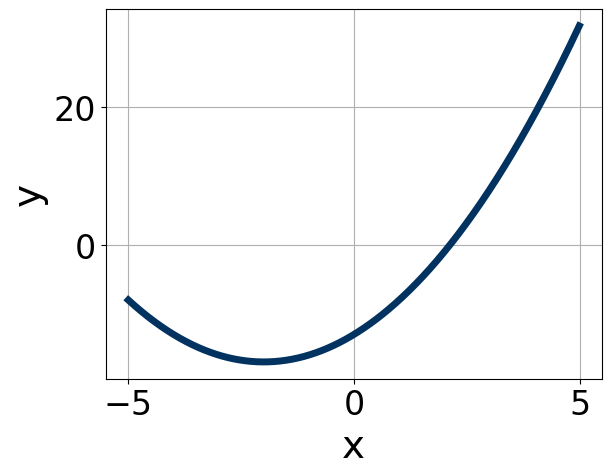
\includegraphics[width=0.3\textwidth]{../Figures/quadraticEquationToGraphBA.png}
\end{center}\begin{enumerate}[label=\Alph*.]
\begin{multicols}{2}
\item 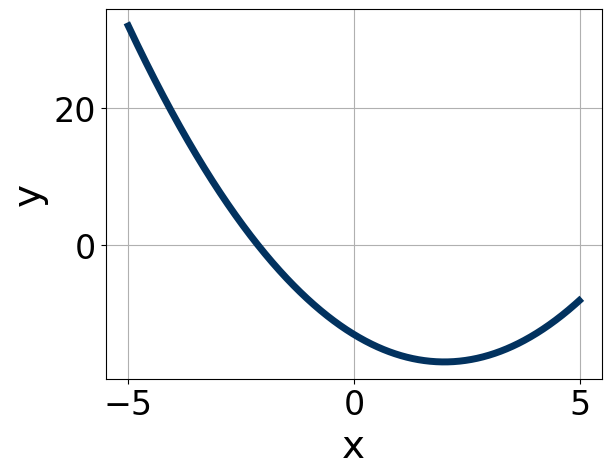
\includegraphics[width = 0.3\textwidth]{../Figures/quadraticEquationToGraphAA.png}
\item 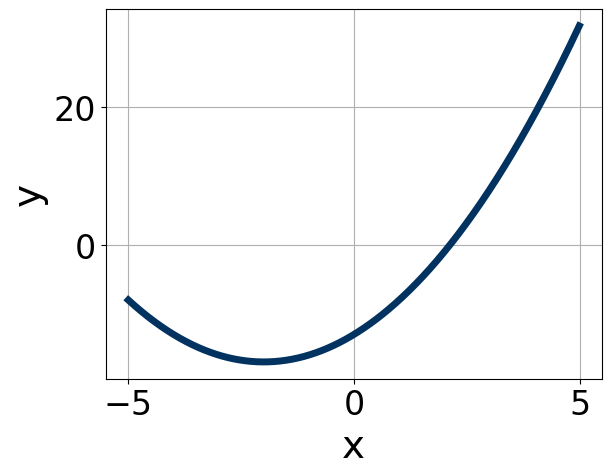
\includegraphics[width = 0.3\textwidth]{../Figures/quadraticEquationToGraphBA.png}
\item 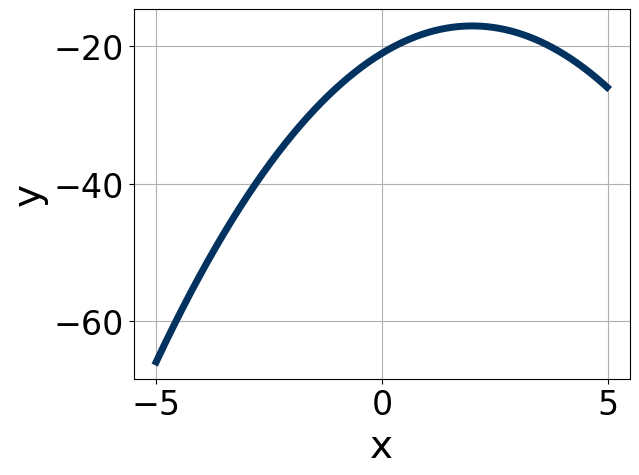
\includegraphics[width = 0.3\textwidth]{../Figures/quadraticEquationToGraphCA.png}
\item 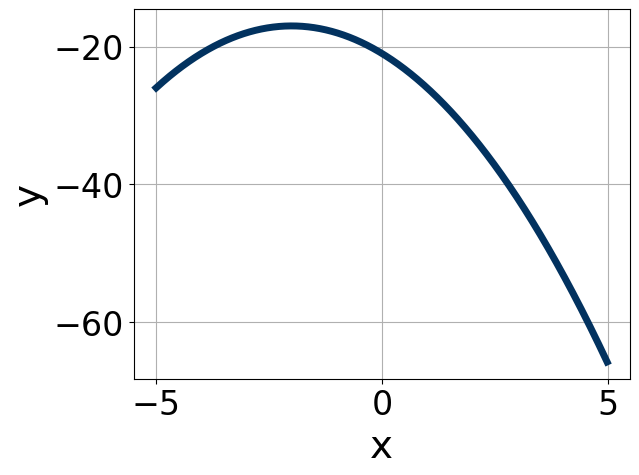
\includegraphics[width = 0.3\textwidth]{../Figures/quadraticEquationToGraphDA.png}
\end{multicols}\item None of the above.\end{enumerate}
\textbf{General Comment:} Remember that Vertex Form is $y = a(x-h)^2+k$, where the vertex is $(h, k)$.
}
\litem{
Find the equation of the line described below. Write the linear equation as $ y=mx+b $ and choose the intervals that contain $m$ and $b$.
\[ \text{Perpendicular to } 5 x - 9 y = 13 \text{ and passing through the point } (4, 8). \]

The solution is \( y = -1.80x + 15.20 \), which is option A.\begin{enumerate}[label=\Alph*.]
\item \( m \in [-3.2, -1.5] \hspace*{3mm} b \in [10.2, 17.2] \)

* $y = -1.80x + 15.20$, which is the correct option.
\item \( m \in [-0.9, 0.5] \hspace*{3mm} b \in [10.2, 17.2] \)

 $y = -0.56x + 15.20$, which corresponds to using the reciprocal slope $(1/m)$.
\item \( m \in [1, 2.1] \hspace*{3mm} b \in [-3.2, 2.8] \)

 $y = 1.80x + 0.80$, which corresponds to using the negative slope.
\item \( m \in [-3.2, -1.5] \hspace*{3mm} b \in [-15.2, -14.2] \)

 $y = -1.80x - 15.20$, which corresponds to using the correct slope and getting the negative $y$-intercept.
\item \( m \in [-3.2, -1.5] \hspace*{3mm} b \in [2, 6] \)

 $y = -1.80x + 4.00$, which corresponds to correct slope and mis-distributing while simplifying to slope-intercept form.
\end{enumerate}

\textbf{General Comment:} Parallel slope is the same and perpendicular slope is opposite reciprocal. Opposite reciprocal means flipping the fraction and changing the sign (positive to negative or negative to positive).
}
\litem{
What is the domain of the function below?
\[ f(x) = \sqrt[7]{-7 x + 8} \]

The solution is \( (-\infty, \infty) \), which is option E.\begin{enumerate}[label=\Alph*.]
\item \( \text{The domain is } (-\infty, a], \text{   where } a \in [0.44, 1.05] \)

$(-\infty, 0.875]$, which corresponds to if the radical had an even power AND using the negative of the correct pivot value.
\item \( \text{The domain is } [a, \infty), \text{   where } a \in [0.86, 1] \)

$[0.875, \infty)$, which corresponds to if the radical had an even power AND reversing the direction of the domain AND using the negative of the correct pivot value.
\item \( \text{The domain is } [a, \infty), \text{   where } a \in [0.93, 2.03] \)

$[1.143, \infty)$, which corresponds to if the radical had an even power AND reversing the direction of the domain.
\item \( \text{The domain is } (-\infty, a], \text{   where } a \in [0.88, 1.46] \)

$(-\infty, 1.143]$, which corresponds to if the radical had an even power.
\item \( (-\infty, \infty) \)

* This is the correct option since the radical has an odd power.
\end{enumerate}

\textbf{General Comment:} Remember that we cannot take the even root of a negative number - this is why the domain is only sometimes restricted! If we have an even root, we solve $-7 x + 8 \geq 0$. Since this is an inequality, remember to flip the inequality if we divide by a negative number.
}
\litem{
Write the equation of the graph presented below in the form $f(x)=ax^2+bx+c$, assuming  $a=1$ or $a=-1$. Then, choose the intervals that $a, b,$ and $c$ belong to.

\begin{center}
    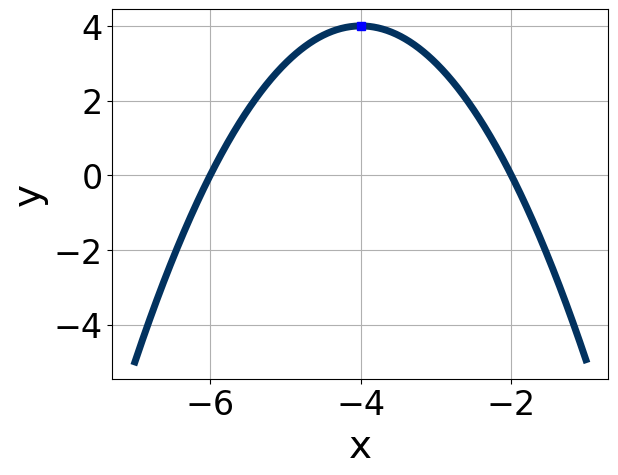
\includegraphics[width=0.5\textwidth]{../Figures/quadraticGraphToEquationA.png}
\end{center}




The solution is \( f(x) = -x^{2} -8 x -12 \), which is option B.\begin{enumerate}[label=\Alph*.]
\item \( a \in [-0.6, 1.1], \hspace*{5mm} b \in [4, 13], \text{ and } \hspace*{5mm} c \in [16, 25] \)

$f(x)=x^{2} +8 x + 20$, which corresponds to making $a$ the opposite sign than it should be.
\item \( a \in [-2.9, 0.7], \hspace*{5mm} b \in [-10, -7], \text{ and } \hspace*{5mm} c \in [-12, -8] \)

* $f(x)=-x^{2} -8 x -12$, which is the correct option.
\item \( a \in [-2.9, 0.7], \hspace*{5mm} b \in [4, 13], \text{ and } \hspace*{5mm} c \in [-12, -8] \)

$f(x)=-x^{2} +8 x -12$, which corresponds to incorrectly using vertex form as $f(x) = a(x+h)^2+k$.
\item \( a \in [-2.9, 0.7], \hspace*{5mm} b \in [4, 13], \text{ and } \hspace*{5mm} c \in [-20, -18] \)

$f(x)=-x^{2} +8 x -20$, which corresponds to incorrectly using vertex form as $f(x) = a(x+h)^2 - k$.
\item \( a \in [-0.6, 1.1], \hspace*{5mm} b \in [-10, -7], \text{ and } \hspace*{5mm} c \in [16, 25] \)

$f(x)=x^{2} -8 x + 20$, which corresponds to incorrectly using vertex form as $f(x) = a(x+h)^2+k$ AND making $a$ the opposite sign than it should be.
\end{enumerate}

\textbf{General Comment:} When the graph is pointing up, $a=1$. When the graph is pointing down, $a=-1$. Be sure to use Vertex Form: $y = a(x-h)^2+k$.
}
\litem{
Which of the following intervals describes the Range of the function below?
\[ f(x) = -\log_2{(x-4)}-8 \]

The solution is \( (\infty, \infty) \), which is option E.\begin{enumerate}[label=\Alph*.]
\item \( (-\infty, a), a \in [7, 14] \)

$(-\infty, 8)$, which corresponds to using the using the negative of vertical shift on $(0, \infty)$.
\item \( [a, \infty), a \in [-4, 3] \)

$[-4, \infty)$, which corresponds to using the negative of the horizontal shift AND including the endpoint.
\item \( (-\infty, a), a \in [-13, -7] \)

$(-\infty, -8)$, which corresponds to using the vertical shift while the Range is $(-\infty, \infty)$.
\item \( [a, \infty), a \in [-2, 7] \)

$[-8, \infty)$, which corresponds to using the flipped Domain AND including the endpoint.
\item \( (-\infty, \infty) \)

*This is the correct option.
\end{enumerate}

\textbf{General Comment:} \textbf{General Comments}: The domain of a basic logarithmic function is $(0, \infty)$ and the Range is $(-\infty, \infty)$. We can use shifts when finding the Domain, but the Range will always be all Real numbers.
}
\litem{
Choose the equation of the function graphed below.

\begin{center}
    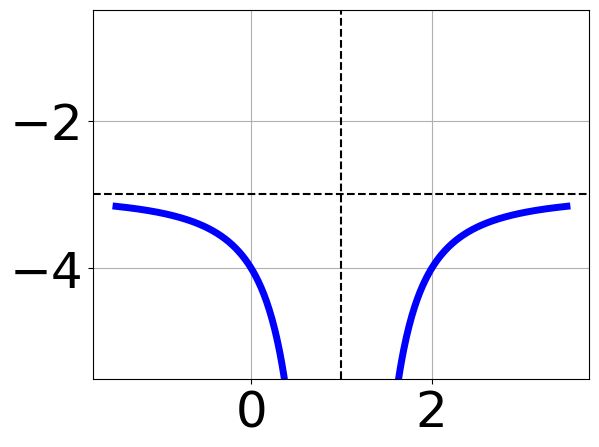
\includegraphics[width=0.5\textwidth]{../Figures/rationalGraphToEquationA.png}
\end{center}




The solution is \( \text{None of the above as it should be } f(x) = \frac{-1}{(x - 1)^2} - 3 \), which is option E.\begin{enumerate}[label=\Alph*.]
\item \( f(x) = \frac{-1}{x + 1} - 3 \)

Corresponds to thinking the graph was a shifted version of $\frac{1}{x}$.
\item \( f(x) = \frac{1}{x - 1} - 3 \)

Corresponds to thinking the graph was a shifted version of $\frac{1}{x}$, using the general form $f(x) = \frac{a}{(x-h)^2}+k$, and the opposite leading coefficient.
\item \( f(x) = \frac{1}{(x - 1)^2} - 3 \)

Corresponds to using the general form $f(x) = \frac{a}{(x-h)^2}+k$ and the opposite leading coefficient.
\item \( f(x) = \frac{-1}{(x + 1)^2} - 3 \)

The $x$-value of the equation does not match the graph.
\item \( \text{None of the above} \)

None of the equation options were the correct equation.
\end{enumerate}

\textbf{General Comment:} Remember that the general form of a basic rational equation is $ f(x) = \frac{a}{(x-h)^n} + k$, where $a$ is the leading coefficient (and in this case, we assume is either $1$ or $-1$), $n$ is the degree (in this case, either $1$ or $2$), and $(h, k)$ is the intersection of the asymptotes.
}
\litem{
Choose the \textbf{smallest} set of Real numbers that the number below belongs to.
\[ -\sqrt{\frac{576}{625}} \]

The solution is \( \text{Rational} \), which is option A.\begin{enumerate}[label=\Alph*.]
\item \( \text{Rational} \)

* This is the correct option!
\item \( \text{Whole} \)

These are the counting numbers with 0 (0, 1, 2, 3, ...)
\item \( \text{Not a Real number} \)

These are Nonreal Complex numbers \textbf{OR} things that are not numbers (e.g., dividing by 0).
\item \( \text{Integer} \)

These are the negative and positive counting numbers (..., -3, -2, -1, 0, 1, 2, 3, ...)
\item \( \text{Irrational} \)

These cannot be written as a fraction of Integers.
\end{enumerate}

\textbf{General Comment:} First, you \textbf{NEED} to simplify the expression. This question simplifies to $-\frac{24}{25}$. 
 
 Be sure you look at the simplified fraction and not just the decimal expansion. Numbers such as 13, 17, and 19 provide \textbf{long but repeating/terminating decimal expansions!} 
 
 The only ways to *not* be a Real number are: dividing by 0 or taking the square root of a negative number. 
 
 Irrational numbers are more than just square root of 3: adding or subtracting values from square root of 3 is also irrational.
}
\litem{
Solve the linear equation below. Then, choose the interval that contains the solution.
\[ \frac{-9x + 9}{8} - \frac{-9x -6}{4} = \frac{9x + 8}{5} \]

The solution is \( x = 1.519 \), which is option C.\begin{enumerate}[label=\Alph*.]
\item \( x \in [9.1, 11.7] \)

 $x = 10.370$, which corresponds to dividing the coefficients in front of x by the denominator rather than dividing BOTH parts of the numerator by the denominator (or removing the fractions through multiplication).
\item \( x \in [-0.5, 0.6] \)

 $x = 0.114$, which corresponds to dividing the second number in the numerator by the denominator rather than dividing BOTH parts of the numerator by the denominator (or removing the fractions through multiplication).
\item \( x \in [0.6, 3.8] \)

* $x = 1.519$, which is the correct option.
\item \( x \in [-5.9, -2.2] \)

 $x = -2.926$, which corresponds to not distributing the negative in front of the second fraction.
\item \( \text{There are no real solutions.} \)

Corresponds to students thinking a fraction means there is no solution to the equation.
\end{enumerate}

\textbf{General Comment:} If you are having trouble with this problem, try to remove a fraction at a time by multiplying each term by the denominator.
}
\litem{
Describe the zero behavior of the zero $x = 4$ of the polynomial below.
\[ f(x) = -5(x + 4)^{8}(x - 4)^{9}(x + 9)^{4}(x - 9)^{5} \]

The solution is the graph below, which is option D.
\begin{center}
    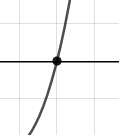
\includegraphics[width=0.3\textwidth]{../Figures/polyZeroBehaviorDA.png}
\end{center}\begin{enumerate}[label=\Alph*.]
\begin{multicols}{2}
\item 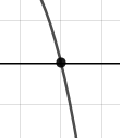
\includegraphics[width = 0.3\textwidth]{../Figures/polyZeroBehaviorAA.png}
\item 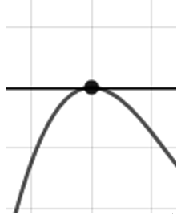
\includegraphics[width = 0.3\textwidth]{../Figures/polyZeroBehaviorBA.png}
\item 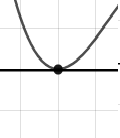
\includegraphics[width = 0.3\textwidth]{../Figures/polyZeroBehaviorCA.png}
\item 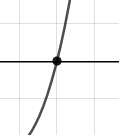
\includegraphics[width = 0.3\textwidth]{../Figures/polyZeroBehaviorDA.png}
\end{multicols}\item None of the above.\end{enumerate}
\textbf{General Comment:} You will need to sketch the entire graph, then zoom in on the zero the question asks about.
}
\litem{
Solve the linear inequality below. Then, choose the constant and interval combination that describes the solution set.
\[ -6x + 4 \geq 7x -3 \]

The solution is \( (-\infty, 0.538] \), which is option B.\begin{enumerate}[label=\Alph*.]
\item \( [a, \infty), \text{ where } a \in [-1.35, -0.39] \)

 $[-0.538, \infty)$, which corresponds to switching the direction of the interval AND negating the endpoint. You likely did this if you did not flip the inequality when dividing by a negative as well as not moving values over to a side properly.
\item \( (-\infty, a], \text{ where } a \in [-0.23, 1.19] \)

* $(-\infty, 0.538]$, which is the correct option.
\item \( [a, \infty), \text{ where } a \in [0.37, 2.04] \)

 $[0.538, \infty)$, which corresponds to switching the direction of the interval. You likely did this if you did not flip the inequality when dividing by a negative!
\item \( (-\infty, a], \text{ where } a \in [-1.81, 0.13] \)

 $(-\infty, -0.538]$, which corresponds to negating the endpoint of the solution.
\item \( \text{None of the above}. \)

You may have chosen this if you thought the inequality did not match the ends of the intervals.
\end{enumerate}

\textbf{General Comment:} Remember that less/greater than or equal to includes the endpoint, while less/greater do not. Also, remember that you need to flip the inequality when you multiply or divide by a negative.
}
\litem{
Simplify the expression below and choose the interval the simplification is contained within.
\[ 2 - 12^2 + 4 \div 8 * 10 \div 3 \]

The solution is \( -140.333 \), which is option B.\begin{enumerate}[label=\Alph*.]
\item \( [-142.6, -140.45] \)

 -141.983, which corresponds to an Order of Operations error: not reading left-to-right for multiplication/division.
\item \( [-141.71, -139.39] \)

* -140.333, this is the correct option
\item \( [147.49, 149.13] \)

 147.667, which corresponds to an Order of Operations error: multiplying by negative before squaring. For example: $(-3)^2 \neq -3^2$
\item \( [145.93, 146.22] \)

 146.017, which corresponds to two Order of Operations errors.
\item \( \text{None of the above} \)

 You may have gotten this by making an unanticipated error. If you got a value that is not any of the others, please let the coordinator know so they can help you figure out what happened.
\end{enumerate}

\textbf{General Comment:} While you may remember (or were taught) PEMDAS is done in order, it is actually done as P/E/MD/AS. When we are at MD or AS, we read left to right.
}
\litem{
Solve the linear inequality below. Then, choose the constant and interval combination that describes the solution set.
\[ \frac{-10}{3} - \frac{7}{7} x > \frac{-4}{9} x - \frac{5}{2} \]

The solution is \( (-\infty, -1.5) \), which is option A.\begin{enumerate}[label=\Alph*.]
\item \( (-\infty, a), \text{ where } a \in [-2.5, 0.5] \)

* $(-\infty, -1.5)$, which is the correct option.
\item \( (-\infty, a), \text{ where } a \in [1.5, 3.5] \)

 $(-\infty, 1.5)$, which corresponds to negating the endpoint of the solution.
\item \( (a, \infty), \text{ where } a \in [0.5, 3.5] \)

 $(1.5, \infty)$, which corresponds to switching the direction of the interval AND negating the endpoint. You likely did this if you did not flip the inequality when dividing by a negative as well as not moving values over to a side properly.
\item \( (a, \infty), \text{ where } a \in [-1.5, 0.5] \)

 $(-1.5, \infty)$, which corresponds to switching the direction of the interval. You likely did this if you did not flip the inequality when dividing by a negative!
\item \( \text{None of the above}. \)

You may have chosen this if you thought the inequality did not match the ends of the intervals.
\end{enumerate}

\textbf{General Comment:} Remember that less/greater than or equal to includes the endpoint, while less/greater do not. Also, remember that you need to flip the inequality when you multiply or divide by a negative.
}
\litem{
Solve the rational equation below. Then, choose the interval(s) that the solution(s) belongs to.
\[ \frac{-7x}{-6x + 6} + \frac{-7x^{2}}{36x^{2} -72 x + 36} = \frac{2}{-6x + 6} \]

The solution is \( \text{There are two solutions: } x = -0.297 \text{ and } x = 1.154 \), which is option D.\begin{enumerate}[label=\Alph*.]
\item \( x \in [1.12,1.42] \)


\item \( x_1 \in [-0.37, -0.13] \text{ and } x_2 \in [0.86,1.01] \)


\item \( x \in [0.92,1.03] \)


\item \( x_1 \in [-0.37, -0.13] \text{ and } x_2 \in [1.13,1.46] \)

* $x = -0.297 \text{ and } x = 1.154$, which is the correct option.
\item \( \text{All solutions lead to invalid or complex values in the equation.} \)


\end{enumerate}

\textbf{General Comment:} Distractors are different based on the number of solutions. Remember that after solving, we need to make sure our solution does not make the original equation divide by zero!
}
\litem{
Simplify the expression below into the form $a+bi$. Then, choose the intervals that $a$ and $b$ belong to.
\[ \frac{36 + 66 i}{5 - 3 i} \]

The solution is \( -0.53  + 12.88 i \), which is option C.\begin{enumerate}[label=\Alph*.]
\item \( a \in [-19, -17.5] \text{ and } b \in [12.5, 14] \)

 $-18.00  + 12.88 i$, which corresponds to forgetting to multiply the conjugate by the numerator and using a plus instead of a minus in the denominator.
\item \( a \in [-1, 0] \text{ and } b \in [437.5, 438.5] \)

 $-0.53  + 438.00 i$, which corresponds to forgetting to multiply the conjugate by the numerator.
\item \( a \in [-1, 0] \text{ and } b \in [12.5, 14] \)

* $-0.53  + 12.88 i$, which is the correct option.
\item \( a \in [6.5, 8.5] \text{ and } b \in [-22.5, -21.5] \)

 $7.20  - 22.00 i$, which corresponds to just dividing the first term by the first term and the second by the second.
\item \( a \in [10.5, 12.5] \text{ and } b \in [6, 7.5] \)

 $11.12  + 6.53 i$, which corresponds to forgetting to multiply the conjugate by the numerator and not computing the conjugate correctly.
\end{enumerate}

\textbf{General Comment:} Multiply the numerator and denominator by the *conjugate* of the denominator, then simplify. For example, if we have $2+3i$, the conjugate is $2-3i$.
}
\litem{
Solve the rational equation below. Then, choose the interval(s) that the solution(s) belongs to.
\[ \frac{6}{-7x + 6} + -9 = \frac{-3}{56x -48} \]

The solution is \( x = 0.768 \), which is option E.\begin{enumerate}[label=\Alph*.]
\item \( x_1 \in [0.6, 0.72] \text{ and } x_2 \in [-0.23,1.77] \)

$x = 0.714 \text{ and } x = 0.768$, which corresponds to getting the correct solution and believing there should be a second solution to the equation.
\item \( x_1 \in [-1.02, -0.9] \text{ and } x_2 \in [-0.23,1.77] \)

$x = -0.946 \text{ and } x = 0.768$, which corresponds to getting the correct solution and believing there should be a second solution to the equation.
\item \( \text{All solutions lead to invalid or complex values in the equation.} \)

This corresponds to thinking $x = 0.768$ leads to dividing by zero in the original equation, which it does not.
\item \( x \in [-1.02,-0.9] \)

$x = -0.946$, which corresponds to not distributing the factor $-7x + 6$ correctly when trying to eliminate the fraction.
\item \( x \in [0.77,3.77] \)

* $x = 0.768$, which is the correct option.
\end{enumerate}

\textbf{General Comment:} Distractors are different based on the number of solutions. Remember that after solving, we need to make sure our solution does not make the original equation divide by zero!
}
\litem{
Solve the equation for $x$ and choose the interval that contains the solution (if it exists).
\[ 3^{5x+3} = 16^{3x-4} \]

The solution is \( x = 5.093 \), which is option A.\begin{enumerate}[label=\Alph*.]
\item \( x \in [3.09, 6.09] \)

* $x = 5.093$, which is the correct option.
\item \( x \in [-0.52, 4.48] \)

$x = 2.478$, which corresponds to distributing the $\ln(base)$ to the first term of the exponent only.
\item \( x \in [-4.5, -0.5] \)

$x = -3.500$, which corresponds to solving the numerators as equal while ignoring the bases are different.
\item \( x \in [-10.19, -6.19] \)

$x = -7.193$, which corresponds to distributing the $\ln(base)$ to the second term of the exponent only.
\item \( \text{There is no Real solution to the equation.} \)

This corresponds to believing there is no solution since the bases are not powers of each other.
\end{enumerate}

\textbf{General Comment:} \textbf{General Comments:} This question was written so that the bases could not be written the same. You will need to take the log of both sides.
}
\litem{
Which of the following intervals describes the Range of the function below?
\[ f(x) = e^{x-1}-8 \]

The solution is \( (-8, \infty) \), which is option A.\begin{enumerate}[label=\Alph*.]
\item \( (a, \infty), a \in [-11, -7] \)

* $(-8, \infty)$, which is the correct option.
\item \( [a, \infty), a \in [-11, -7] \)

$[-8, \infty)$, which corresponds to including the endpoint.
\item \( (-\infty, a], a \in [8, 11] \)

$(-\infty, 8]$, which corresponds to using the negative vertical shift AND flipping the Range interval AND including the endpoint.
\item \( (-\infty, a), a \in [8, 11] \)

$(-\infty, 8)$, which corresponds to using the negative vertical shift AND flipping the Range interval.
\item \( (-\infty, \infty) \)

This corresponds to confusing range of an exponential function with the domain of an exponential function.
\end{enumerate}

\textbf{General Comment:} \textbf{General Comments}: Domain of a basic exponential function is $(-\infty, \infty)$ while the Range is $(0, \infty)$. We can shift these intervals [and even flip when $a<0$!] to find the new Domain/Range.
}
\litem{
First, find the equation of the line containing the two points below. Then, write the equation as $ y=mx+b $ and choose the intervals that contain $m$ and $b$.
\[ (-7, 11) \text{ and } (9, 3) \]

The solution is \( y = -0.5x + 7.5 \), which is option D.\begin{enumerate}[label=\Alph*.]
\item \( m \in [-1.2, -0.2] \hspace*{3mm} b \in [-7, -2] \)

 $y = -0.5x -6$, which corresponds to using the correct slope/equation but not distributing correctly using the second point.
\item \( m \in [-1.2, -0.2] \hspace*{3mm} b \in [17, 22] \)

 $y = -0.5x + 18$, which corresponds to using the correct slope/equation but not distributing correctly using the first point.
\item \( m \in [-1.2, -0.2] \hspace*{3mm} b \in [-7.5, -6.5] \)

 $y = -0.5x -7.5$, which corresponds to using the correct slope and getting the negative y-intercept.
\item \( m \in [-1.2, -0.2] \hspace*{3mm} b \in [5.5, 9.5] \)

* $y = -0.5x + 7.5$, which is the correct option.
\item \( m \in [-0.4, 3.2] \hspace*{3mm} b \in [-3.5, 6.5] \)

 $y = 0.5x -1.5$, which corresponds to using the negative slope and the correct equation.
\end{enumerate}

\textbf{General Comment:} Remember to keep your points in order when plugging in to the slope formula.
}
\litem{
Solve the linear inequality below. Then, choose the constant and interval combination that describes the solution set.
\[ -6 + 7 x < \frac{33 x - 3}{4} \leq -3 + 6 x \]

The solution is \( (-4.20, -1.00] \), which is option B.\begin{enumerate}[label=\Alph*.]
\item \( (-\infty, a] \cup (b, \infty), \text{ where } a \in [-4.2, -3.2] \text{ and } b \in [-2.6, -0.1] \)

$(-\infty, -4.20] \cup (-1.00, \infty)$, which corresponds to displaying the and-inequality as an or-inequality AND flipping the inequality.
\item \( (a, b], \text{ where } a \in [-6.2, -1.2] \text{ and } b \in [-1.7, -0.7] \)

* $(-4.20, -1.00]$, which is the correct option.
\item \( [a, b), \text{ where } a \in [-4.2, -3.2] \text{ and } b \in [-4, 0] \)

$[-4.20, -1.00)$, which corresponds to flipping the inequality.
\item \( (-\infty, a) \cup [b, \infty), \text{ where } a \in [-4.2, -0.2] \text{ and } b \in [-1, 0] \)

$(-\infty, -4.20) \cup [-1.00, \infty)$, which corresponds to displaying the and-inequality as an or-inequality.
\item \( \text{None of the above.} \)


\end{enumerate}

\textbf{General Comment:} To solve, you will need to break up the compound inequality into two inequalities. Be sure to keep track of the inequality! It may be best to draw a number line and graph your solution.
}
\end{enumerate}

\end{document}